\chapter{Les atomes de Rydberg circulaires en interaction : vers un simulateur quantique}
\label{chapter:circsim}

%Intro : pourquoi envisager les Rydberg circulaires comme plateforme de simulation ?
\noindent La bonne compréhension des interactions entre atomes de Rydberg sphériques permet d'imaginer leur utilisation comme plateforme de simulation quantique.
%Les simulations menées par Thanh Long Nguyen \cite{PHD_NGUYEN} montrent la difficulté de la préparation déterministe d'un ensemble d'atomes de Rybderg adapté à cette fin.
Un premier obstacle majeur s'oppose à cette idée.
La préparation d'une chaîne régulière d'atomes de Rydberg dans le niveau $\mathrm{60S}$ en s'appuyant sur le mécanisme d'excitation facilitée paraît difficile \cite{PHD_NGUYEN}.

Nous présentons ici une proposition de simulateur quantique à partir d'atomes de Rydberg circulaires piégés par laser.
Cette proposition est formulée en détail dans la thèse de Thanh Long Nguyen \cite{PHD_NGUYEN}.
L'article \cite{ENS_PRE_CIRCSIM} en reprend les points essentiels.

Le simulateur proposé repose sur les interactions entre atomes de Rydberg circulaires.
Nous dirons quelques mots de celles-ci en présence d'un champ électrique et d'un champ magnétique externe, en complément de \ref{subsec:interac50C_I}.
Ces interactions permettent de simuler le hamiltonien \og XXZ \fg{} d'une chaîne de spins $1/2$, que nous présenterons.
Nous terminerons ce chapitre avec une discussion des points techniques nécessaires à la réalisation d'un tel simulateur : le piégeage laser des atomes de Rydberg circulaires, l'allongement de leur durée de vie par inhibition de l'émission spontanée et la préparation déterministe d'une chaîne de tels atomes.


\section{Les interactions dipôle-dipôle entre atomes de Rydberg circulaires}
\noindent Les interactions dipôle-dipôle entre atomes de Rydberg circulaires sont au c\oe ur de notre proposition de simulateur.
Comme nous l'avons mentionné en \ref{subsec:interac50C_I}, la présence d'un champ électrique externe permet de fixer un axe de quantification, et donc de fixer l'orientation des orbites de grand moment cinétique.
Dans la présente discussion, nous considérerons que les atomes de Rydberg circulaires sont placés sur un axe $Ox$, perpendiculaire au champ directeur selon $Oz$, tels que représentés en figure \eqref{fig:double_torus}.

%\subsection{La structure des niveaux atomiques et des niveaux de paire près des circulaires}
\subsection{Les niveaux circulaires et leurs interactions en présence de champs électrique et magnétique}
\noindent En présence d'un champ électrique, les niveaux à grand moment cinétique d'une même multiplicité voient leur dégénérescence partiellement levée.
Le diagramme d'énergie de ces niveaux est représenté en figure (\ref{fig:ener_StarknC_nCnC}a)).
Le niveau circulaire est noté $\ket{\mathrm{nC}}$ et les deux niveaux \og elliptiques \fg{} voisins sont notés $\ket{\mathrm{nE^{\pm}}} = \ket{n,m=n-2,k=\pm1}$.
De la même façon, les niveaux de $m=n-3$ sont notés $\ket{\mathrm{nEE^0}} = \ket{n,m=n-3,k=0}$ et $\ket{\mathrm{nEE^{\pm}}} = \ket{n,m=n-3,k=\pm 2}$.
%
\begin{figure}[!h]
\centering
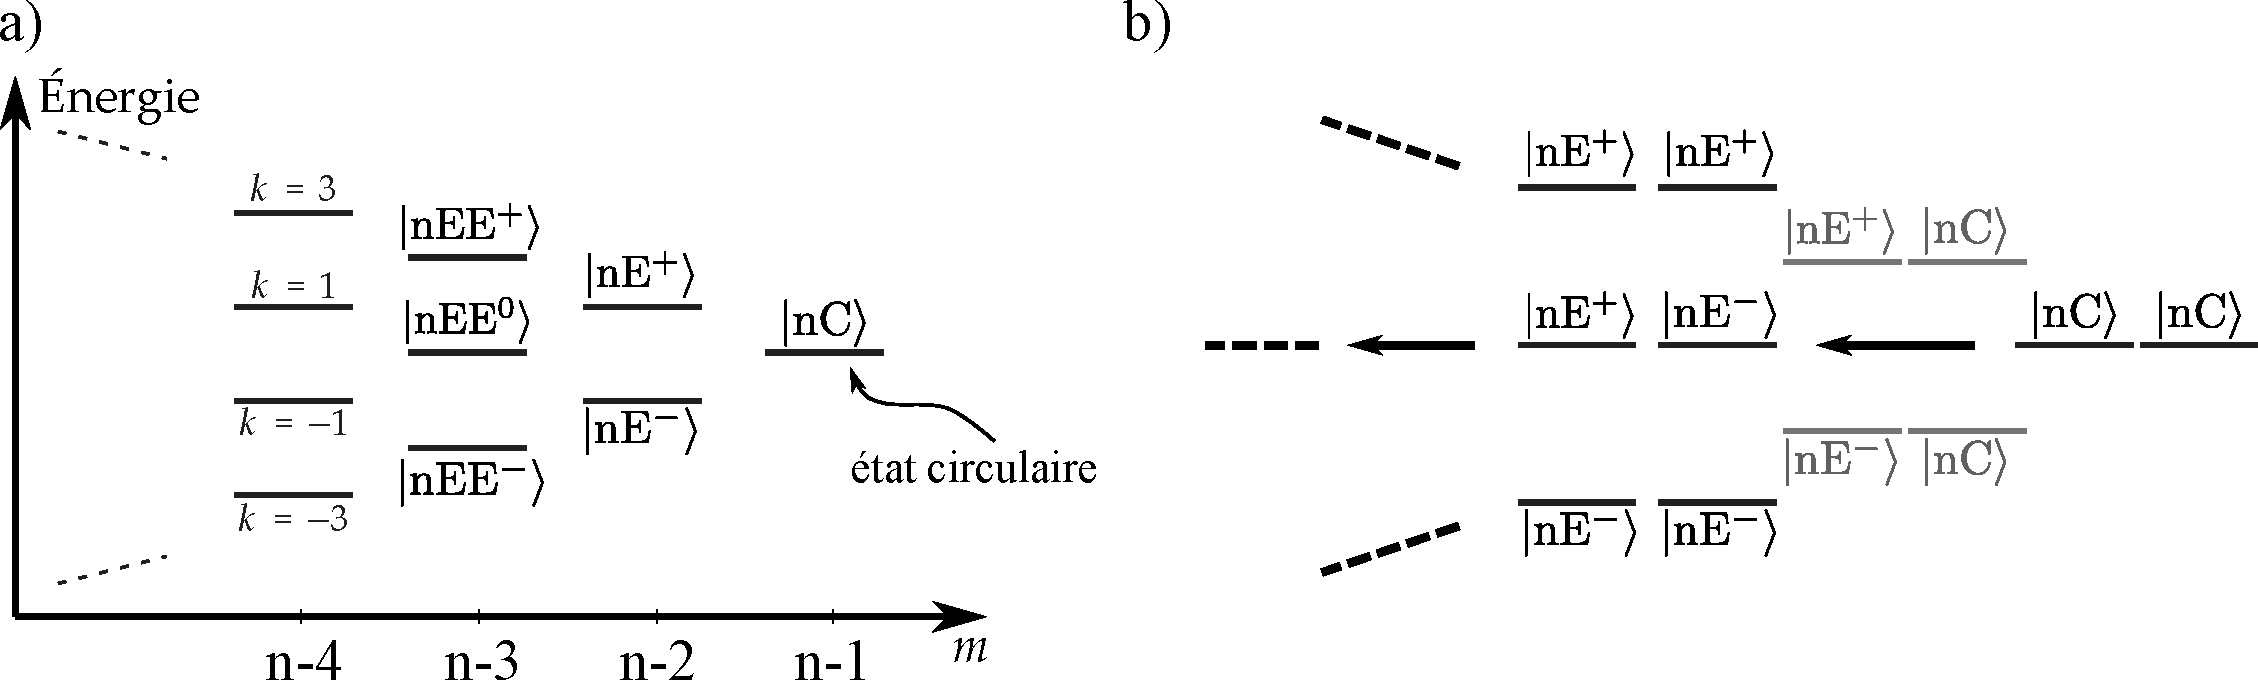
\includegraphics[width=\linewidth]{figures/circsim/diagram_nC_nCnC}
\caption[Diagammre d'énergie des niveaux proches du $\mathrm{50C}$]{
\textbf{a)} Diagramme d'énergie des niveaux proches de $\mathrm{nC}$, en présence d'un champ électrique.
\textbf{b)} Diagramme d'énergie des niveaux de paire proches de $\ket{\mathrm{nC}}\ket{\mathrm{nC}}$ en présence d'un champ électrique.
Le champ électrique est dirigé selon $Oz$, perpendiculaire au vecteur qui sépare les deux atomes de la paire,  dirigé selon $Ox$.
}
\label{fig:ener_StarknC_nCnC}
\end{figure}

%\noindent Il est utile de rappeler ici la forme analytique de l'énergie des niveaux proches du circulaire en présence d'un champ électrique $\vec{F}$, tirée de l'équation \eqref{eq:Stark_circular} :
%%
%\begin{equation}
%\label{eq:Stark_nC_explicit}
%\begin{aligned}
%E_{\mathrm{nC}} &= -\frac{1}{2n^2} - \frac{1}{16}n^4(8n^2+18n+10)|\vec{F}|^2\\
%&=-\frac{1}{2n^2}+\alpha_{\mathrm{nC}}|\vec{F}|^2 ,\\
%E_{\mathrm{nE^{\pm}}} &= -\frac{1}{2n^2} \pm \frac{3n}{2}|\vec{F}| -  \frac{1}{16}n^4(8n^2+36n-20)|\vec{F}|^2 \\
%&=-\frac{1}{2n^2} \pm \frac{3n}{2} +\alpha_{\mathrm{nE^{\pm}}}|\vec{F}|^2 ,
%\end{aligned}
%\end{equation}
%%
%où les coefficients $\alpha$ d'effet Stark quadratique sont introduits pour simplifier l'écriture.

Il s'agit maintenant de comprendre quelle forme prend l'interaction dipôle-dipôle dans le cas présent.
Replaçons nous dans le cas de deux atomes séparés d'une distance $r$.
En \ref{sec:interacting_rydbergs} nous avions exprimé, en l'absence de champ électrique extérieur, le hamiltonien de couplage dans la base des harmoniques sphériques (cf. équation \eqref{eq:Vdd_rr1r2}).
De plus, l'axe de quantification était alors déterminé par le vecteur séparant la paire d'atomes en interaction.
Ici au contraire, l'axe de quantification est déterminé par le champ électrique extérieur, selon $Oz$ donc, et le vecteur séparant les atomes sont situés sur l'axe $Ox$, à des positions $\vec{r_1},\vec{r_2}$ respectivement.
Le hamiltonien d'interaction dipôle-dipôle prend alors la forme
\begin{equation}
\label{eq:dipdip_nC}
\hat{V}_{dd} = -\frac{q^2\hat{r_1} \hat{r_2}}{3\epsilon_0 r^3}
\left[ Y_1^0 Y_1^0 + \frac{1}{2} \left( Y_1^{+1}Y_1^{-1} + Y_1^{-1}Y_1^{+1} \right)
- \frac{3}{2} \left(  Y_1^{+1}Y_1^{+1} + Y_1^{-1}Y_1^{-1} \right) \right],
\end{equation}
où les $Y_l^m$ sont les harmoniques sphériques.
On remarque ici que le moment magnétique total de la paire atomique n'est plus nécessairement conservé par l'interaction dipôle-dipôle.
Ainsi le niveau de paire $\ket{\mathrm{nC},\mathrm{nC}}$ se trouve couplé de façon quasi résonante avec le niveau de paire $\ket{\mathrm{nE^+},\mathrm{nE^-}}$, lui-même couplé aux niveaux de paire $\ket{\mathrm{nEE^+},\mathrm{nEE^-}}$ et $\ket{\mathrm{nEE^0},\mathrm{nEE^0}}$, et ainsi de suite.
La figure (\ref{fig:ener_StarknC_nCnC} b) représente les niveaux de paire proches du niveau $\ket{\mathrm{nC},\mathrm{nC}}$ en présence d'un champ électrique.

Ces couplages quasi résonants, dès lors que la distance entre les atomes est suffisamment petite, perturbent le niveau $\ket{\mathrm{nC,nC}}$ en le mélangeant aux niveaux de paires d'énergie suffisamment proche.
C'est ce que nous avions vu en \ref{subsec:interac50C_I} : en figure \eqref{fig:VdW_50C50C_1Vcm}, lorsque les deux atomes de la paire sont plus proches que $\SI{10}{\um}$, l'état propre du hamiltonien complet s'éloigne du niveau non perturbé $\ket{\mathrm{50C,50C}}$.
Cet effet de mélange a plusieurs conséquences néfastes.
Tout d'abord, l'interaction dipôle-dipôle ne peut plus être simplement approximée par un déplacement d'énergie en $1/r^6$ entre deux atomes dans un niveau de paire $\ket{n,k,m}\ket{n,k,m}$.
De plus, le mélange avec les niveaux elliptiques réduit le temps de vie du niveau de paire à deux atomes circulaires.
En effet, les niveaux elliptiques peuvent être deséxcités par des transitions $\pi$ vers la multiplicité inférieure alors que le niveau circulaire ne peut être deséxcité que par une transition $\sigma^+$.
Or le dispositif d'inhibition de l'émission spontanée que nous proposons, qui sera discuté en \ref{subsec:inhibition}, ne peut inhiber que l'émission spontanée $\sigma^+$.
Ainsi donc, le gain de temps de vie permis par ce dispositif est perdu dès lors que des transitions $\pi$ sont accessibles.

Afin de contourner cette difficulté, il faut trouver un moyen de lever la dégénérescence des niveaux de paire non perturbés représentés en figure (\ref{fig:ener_StarknC_nCnC} b).
Deux paramètres sont à notre disposition pour ce faire.
Le premier est la valeur du champ électrique.
Les niveaux de paire non perturbés sont d'autant plus distants en énergie que le champ électrique est élevé.
Cependant, la variation du champ électrique nous servira à faire varier l'interaction elle-même comme nous l'expliquerons en \ref{subsec:tunability}.
Le second moyen dont nous disposons est l'imposition d'un champ magnétique extérieur $B_z$, orienté selon $Oz$, qui déplacera les niveaux par effet Zeeman.

Le hamiltonien Zeeman pour un état circulaire prend alors la forme%\footnote{
%on néglige le spin de l'électron
%}
\begin{equation}
\label{eq:H_Zeeman}
\hat{H}_Z = \mu_B g_l~\hat{\vec{L}}\cdot\vec{B} = \mu_B g_l\hat{L}_zB_z,
%\frac{\mu_B g_l}{\hbar}~\hat{\vec{L}}\cdot\vec{B} = \frac{\mu_B g_l}{\hbar}\hat{L}_zB_z,
\end{equation}
où $\mu_B$ est le magnéton de Bohr et $g_l$ le facteur de Landé pour le nombre quantique orbital $l$.
Dans la mesure où l'on néglige le spin de l'électron, qui est très petit devant $l$ ($s=1/2 \ll l\simeq 50$), le facteur de Landé peut être approximé à $g_l \simeq -1$.
Ce hamiltonien conserve le nombre quantique magnétique $m$, qui n'est autre que la valeur propre de l'opérateur $\hat{L_z}$\footnote{
Si le champ magnétique avait des composantes non nulles selon $Ox$ et $Oy$, celles-ci coupleraient des états de $m$ différents.}.
Tant que le champ magnétique $B_z$ reste suffisamment petit, l'effet Zeeman agit comme une perturbation au premier ordre du hamiltonien \eqref{eq:hamilt_Stark} de l'atome dans un champ électrique.
La seule conséquence de l'effet Zeeman sur le niveau $\ket{n,m,k}$ sera un déplacement d'énergie
\begin{equation}
\label{eq:Zeeman_shift}
\Delta E_Z (n,m,k) = \braket{n,m,k|g_l \hat{L}_z | n,m,k}\cdot \mu_B B_z \simeq m\cdot \mu_B B_z = \Delta E_Z (m).
\end{equation}
Le niveau de paire $\ket{n,m,k ; n,m',k'}$ sera déplacé de la somme du déplacement d'énergie de $\ket{n,m,k}$ et $\ket{n,m',k'}$, soit $(m+m')\mu_B B_z$.

En tenant compte de l'effet Stark (cf. équation \eqref{eq:Stark_circular}) et de l'effet Zeeman perturbatif, on obtient les énergies suivantes pour les niveaux circulaires et elliptiques de la multiplicité $n$ :
\begin{equation}
\label{eq:ener_nC_ZeeStark}
\begin{aligned}
E_{\mathrm{nC}}/2E_I &= -\frac{1}{2n^2} - \frac{1}{16}n^4(8n^2+18n+10)|\vec{F}|^2 \left(\frac{ea_0}{2E_I} \right)^2 + (n-1)\mu_B B_z \\
&= -\frac{1}{2n^2} - \alpha_{\mathrm{nC}}|\vec{F}|^2 + (n-1)\mu_B B_z ,\\
E_{\mathrm{nE^{\pm}}}/2E_I &= -\frac{1}{2n^2} \pm \frac{3n}{2}|\vec{F}|\frac{ea_0}{2E_I} - \frac{1}{16}n^4(8n^2+36n-20)|\vec{F}|^2\left(\frac{ea_0}{2E_I} \right)^2 + (n-2)\mu_B B_z \\
&= -\frac{1}{2n^2} \pm \frac{ea_0}{2E_I}\frac{3n}{2}|\vec{F}| +\alpha_{\mathrm{nE^{\pm}}}|\vec{F}|^2 + (n-2)\mu_B B_z,
\end{aligned}
\end{equation}
où les coefficients $\alpha$ d'effet Stark quadratique sont introduits pour simplifier l'écriture.

Appliquons les équations \eqref{eq:ener_nC_ZeeStark} à l'exemple des états de paire non perturbés $\ket{\mathrm{50C,50C}}$ et $\ket{\mathrm{50E^+,50E^-}}$.
Dans les conditions du paragraphe \ref{subsec:interac50C_I}, c'est-à-dire sous $\SI{1}{\V/cm}$ et sans champ magnétique, la distance en énergie entre ces deux états de paire est de $\Delta_E = h\times\SI{169}{\kHz}$.
Si l'on ajoute un champ magnétique $B_z$ de $\SI{10}{\gauss}=\SI{1}{\milli\tesla}$, la distance en énergie devient $\Delta E = h\times \SI{28.17}{\MHz}$, soit presque $\SI{200}{}$ fois plus.
Un faible champ magnétique nous permet ainsi de lever la dégénérescence entre les niveaux de  paire voisins de $\ket{\mathrm{nC,nC}}$.

\subsection{Forme générale de l'interaction et choix des niveaux}
\noindent Dans les condition que nous venons d'établir il nous est possible de calculer l'interaction dipôle-dipôle entre deux atomes circulaires, tout en limitant la perturbation de ces niveaux qui serait due à un couplage résonant.
Ce calcul s'effectue de la même façon qu'en \ref{sec:interacting_rydbergs}, en diagonalisant le hamiltonien complet de la paire atomique\footnote{
La même méthode permet tout aussi bien de calculer l'interaction entre deux atomes dans des niveaux différents, de même qu'en \ref{sec:interacting_rydbergs}.
}.
Ce hamiltonien complet s'écrit
\begin{equation}
\label{eq:hamilt_Vdd_ZeeStark}
\begin{aligned}
\hat{H} &= \hat{H}_1 + \hat{H}_2 + \hat{V}_{dd}(\vec{r}) \\
 &= \hat{H}_{0,1} + \hat{H}_{0,2} + \hat{H}_{S,1} + \hat{H}_{S,2} + \hat{H}_{Z,1} + \hat{H}_{Z,2} + \hat{V}_{dd}(\vec{r}),
\end{aligned}
\end{equation}
où $\hat{H}_{0,i},\hat{H}_{S,i},\hat{H}_{Z,i}$ sont respectivement les hamiltoniens libre, Stark et Zeeman de l'atome $i$ et $\hat{H}_i$ le hamiltonien total de l'atome $i$ isolé.

Nous pouvons, ici encore, écrire l'interaction entre un atome dans le niveau $\mathrm{nC}$ et un atome dans le niveau $\mathrm{n'C}$ comme un hamiltonien effectif
\begin{equation}
V_{eff} = \left(\begin{array}{cc}
C_{\mathrm{nC},\mathrm{n'C}} & A_{\mathrm{nC},\mathrm{n'C}} \\
A_{\mathrm{nC},\mathrm{n'C}} & C_{\mathrm{nC},\mathrm{n'C}},
\end{array} \right)
\end{equation}
où $C_{\mathrm{nC},\mathrm{n'C}}$ et $A_{\mathrm{nC},\mathrm{n'C}}$ sont respectivement les termes d'interaction directe et d'échange entre les niveaux $\mathrm{nC}$ et $\mathrm{n'C}$.
De manière générale, ces termes se décomposent en une composante \og van der Waals \fg{} en $1/r^6$ et une composante de couplage direct en $1/r^3$.
De plus, ils dépendront désormais fortement des champs électrique et magnétique imposés.

%\subsection{Choix du niveau 50-48 et courbes d'interaction}


\section{Le hamiltonien $XXZ$ simulé}
	\subsection{Mise sous forme XXZ}
	\subsection{"Tunabilité" des interactions}\label{subsec:tunability}
		Comment justifier le domaine de champs électrique et magnétique statiques dans lequel on se place, avant d'avoir parlé du problème de la durée de vie ??
	\subsection{Quelle physique ? Diagramme de phase}

\section{Principes techniques du simulateur}
	\subsection{Piégeage laser des Rydberg circulaires}
	\subsection{Préservation des états de Rydberg}\label{subsec:inhibition}
		\subsubsection*{Temps de vie dans l'espace libre}
		\subsubsection*{Inhibition de l'émission spontanée}
		\subsubsection*{Problème du mixing et solution}
	\subsection{Préparation déterministe d'une chaîne}

\newpage
Reprendre le PRX